\newpage
\begin{center}
  \textbf{\large 4 Методические указание на основе результатов экспериментов}
\end{center}
\refstepcounter{chapter}
\addcontentsline{toc}{chapter}{4 Методические указание на основе результатов экспериментов}
После проведенных экспериментов можно сформировать представленные на рисунках \ref{fig:fps_hota_n320}-\ref{fig:fps_hota_s512} сводные таблицы производительности и качества работы различных алгоритмов на Raspberry PI5 с внешним TPU Google Coral.

На основании полученных данных можно сформулировать следующие рекомендации:
\begin{itemize}
  \item с использованием TPU возможно запустить современные алгоритмы отслеживания объектов на видеоизображениях, но с падением метрик качества до уровня примерно 2020 года;
  \item за счет более высокой скорости работы yolov8n может успевать работать на размере изображения 512, что дает качество лучше чем yolov8s на 312. При этом yolov8s на 512 начинает работать хуже из-за сильной просадки в скорости работы;
  \item в общем случае ByteTrack зарекомендовал себя лучше всего. Благодаря нечувствительности к увеличению количества отслеживаемых объектов и общей легковесности, он работает в разы быстрее, за счет чего имеет большое преимущество перед алгоритмами, основывающимися на ReID-моделях; 
  \item OC-SORT обладает всеми теми же плюсами, что и ByteTrack, но работает немного хуже. Его использование не рекомендуется, так как ByteTrack всегда чуть лучше.
  \item два алгоритма -- ImprAssOC и StrongSORT в паре с ReID-моделью OSNet X0.25 -- дают наибольшие показатели HOTA, несмотря на низкую скорость работы. Они рекомендуются к использованию в задачах, где количество отслеживаемых объектов не превышает 5, а так же скорость передвижения объектов в кадре относительно невысока;
  \item BoT-SORT и Deep OC-SORT в паре с ReID-моделью OSNet X0.25 дают показатели качества ниже, чем быстрый ByteTrack. Их использование не рекомендуется.
\end{itemize}

\begin{figure}[ht]
  \centering
  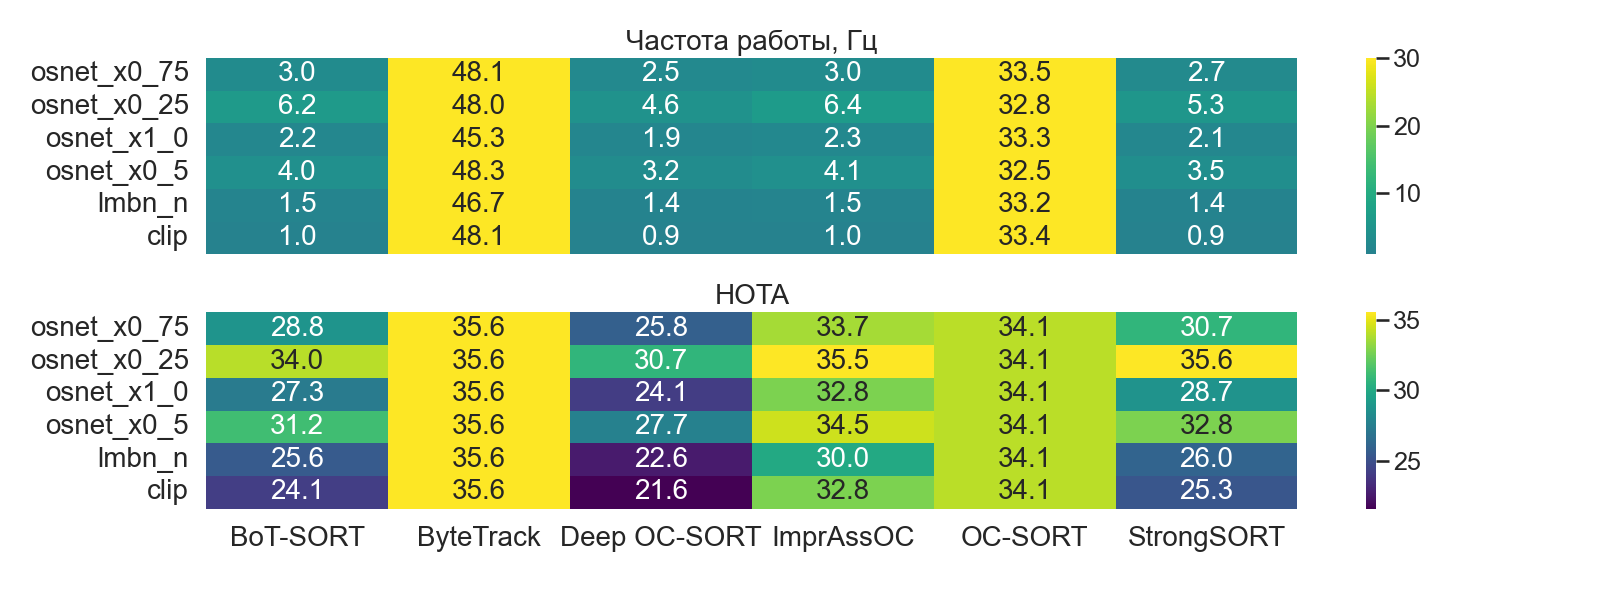
\includegraphics[width=1\textwidth]{./plots/heatmap_fps_hota_vs_tracker_reid/heatmap_fps_hota_yolov8n_size320.png}
  \caption{Таблица производительности и метрики HOTA для yolov8n с размером изображения 320}
  \label{fig:fps_hota_n320}
\end{figure}

\begin{figure}[ht]
  \centering
  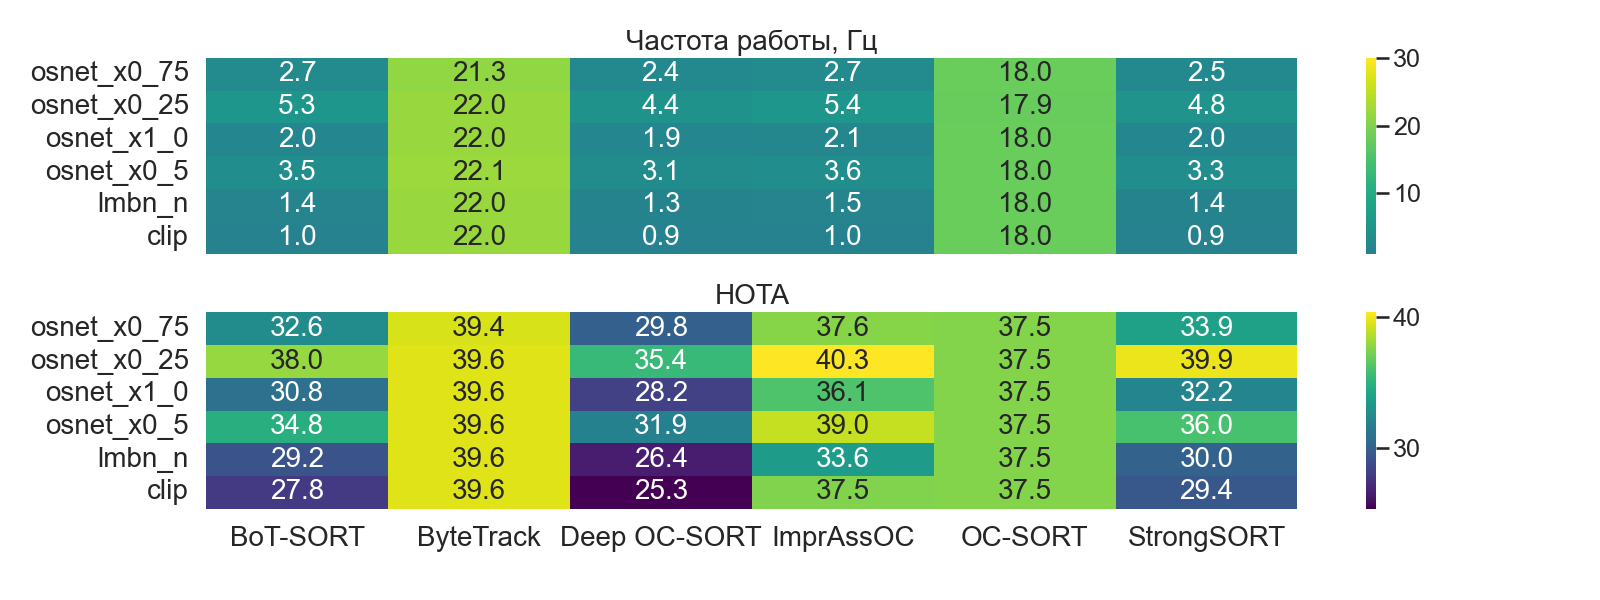
\includegraphics[width=1\textwidth]{./plots/heatmap_fps_hota_vs_tracker_reid/heatmap_fps_hota_yolov8n_size512.png}
  \caption{Таблица производительности и метрики HOTA для yolov8n с размером изображения 512}
  \label{fig:fps_hota_n512}
\end{figure}


\begin{figure}[ht]
  \centering
  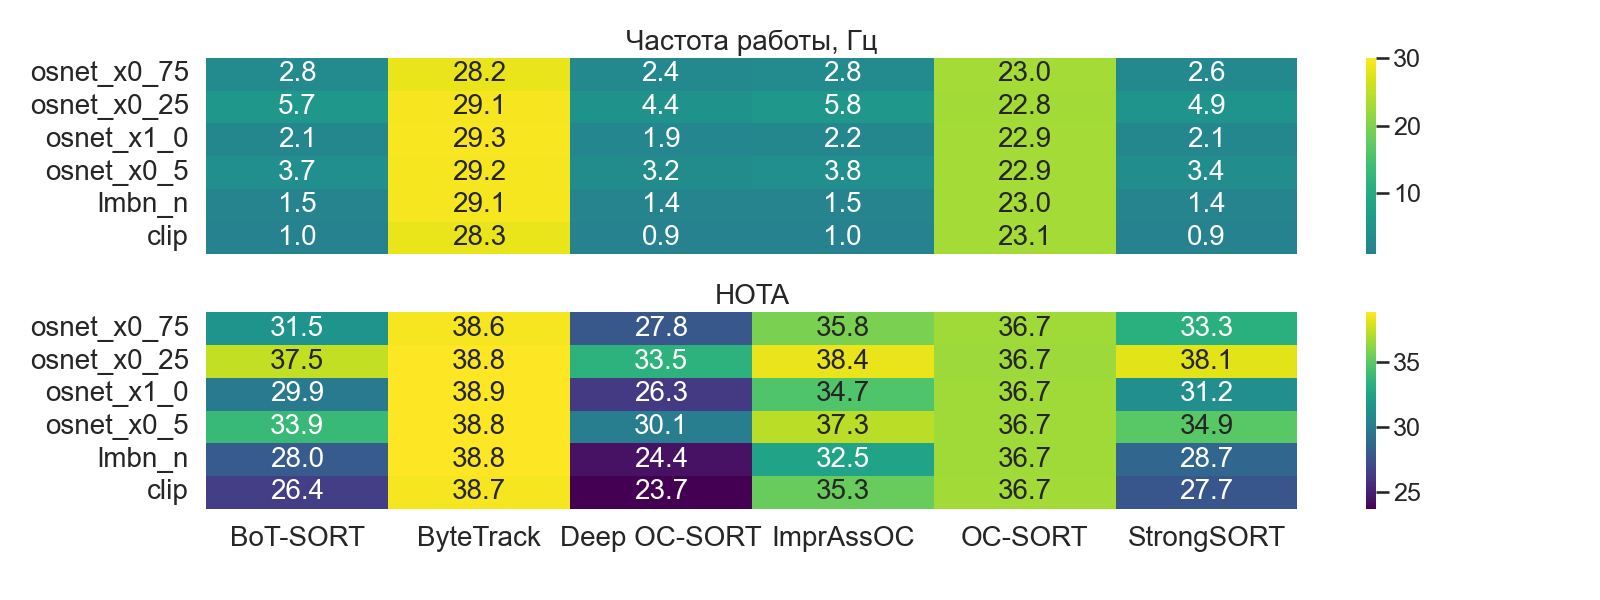
\includegraphics[width=1\textwidth]{./plots/heatmap_fps_hota_vs_tracker_reid/heatmap_fps_hota_yolov8s_size320.png}
  \caption{Таблица производительности и метрики HOTA для yolov8s с размером изображения 320}
  \label{fig:fps_hota_s320}
\end{figure}

\begin{figure}[ht]
  \centering
  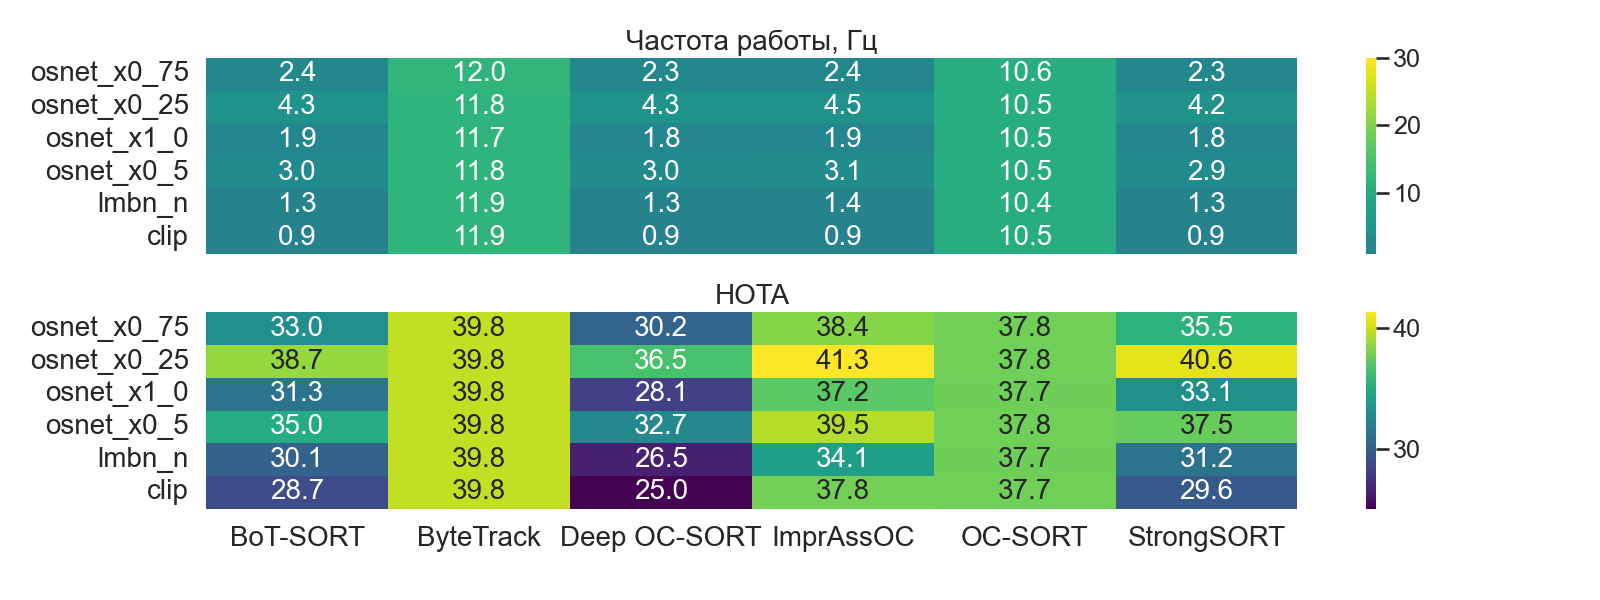
\includegraphics[width=1\textwidth]{./plots/heatmap_fps_hota_vs_tracker_reid/heatmap_fps_hota_yolov8s_size512.png}
  \caption{Таблица производительности и метрики HOTA для yolov8s с размером изображения 512}
  \label{fig:fps_hota_s512}
\end{figure}

% \section{Выбор разрешения видеоизображения}

% \section{Выбор размера сети классификатора}


% \section{Выводы по главе}
